\documentclass[]{article}
\usepackage{lmodern}
\usepackage{amssymb,amsmath}
\usepackage{ifxetex,ifluatex}
\usepackage{fixltx2e} % provides \textsubscript
\ifnum 0\ifxetex 1\fi\ifluatex 1\fi=0 % if pdftex
  \usepackage[T1]{fontenc}
  \usepackage[utf8]{inputenc}
\else % if luatex or xelatex
  \ifxetex
    \usepackage{mathspec}
  \else
    \usepackage{fontspec}
  \fi
  \defaultfontfeatures{Ligatures=TeX,Scale=MatchLowercase}
\fi
% use upquote if available, for straight quotes in verbatim environments
\IfFileExists{upquote.sty}{\usepackage{upquote}}{}
% use microtype if available
\IfFileExists{microtype.sty}{%
\usepackage{microtype}
\UseMicrotypeSet[protrusion]{basicmath} % disable protrusion for tt fonts
}{}
\usepackage[margin=1in]{geometry}
\usepackage{hyperref}
\hypersetup{unicode=true,
            pdftitle={R: Importación de datos},
            pdfborder={0 0 0},
            breaklinks=true}
\urlstyle{same}  % don't use monospace font for urls
\usepackage{color}
\usepackage{fancyvrb}
\newcommand{\VerbBar}{|}
\newcommand{\VERB}{\Verb[commandchars=\\\{\}]}
\DefineVerbatimEnvironment{Highlighting}{Verbatim}{commandchars=\\\{\}}
% Add ',fontsize=\small' for more characters per line
\usepackage{framed}
\definecolor{shadecolor}{RGB}{248,248,248}
\newenvironment{Shaded}{\begin{snugshade}}{\end{snugshade}}
\newcommand{\KeywordTok}[1]{\textcolor[rgb]{0.13,0.29,0.53}{\textbf{#1}}}
\newcommand{\DataTypeTok}[1]{\textcolor[rgb]{0.13,0.29,0.53}{#1}}
\newcommand{\DecValTok}[1]{\textcolor[rgb]{0.00,0.00,0.81}{#1}}
\newcommand{\BaseNTok}[1]{\textcolor[rgb]{0.00,0.00,0.81}{#1}}
\newcommand{\FloatTok}[1]{\textcolor[rgb]{0.00,0.00,0.81}{#1}}
\newcommand{\ConstantTok}[1]{\textcolor[rgb]{0.00,0.00,0.00}{#1}}
\newcommand{\CharTok}[1]{\textcolor[rgb]{0.31,0.60,0.02}{#1}}
\newcommand{\SpecialCharTok}[1]{\textcolor[rgb]{0.00,0.00,0.00}{#1}}
\newcommand{\StringTok}[1]{\textcolor[rgb]{0.31,0.60,0.02}{#1}}
\newcommand{\VerbatimStringTok}[1]{\textcolor[rgb]{0.31,0.60,0.02}{#1}}
\newcommand{\SpecialStringTok}[1]{\textcolor[rgb]{0.31,0.60,0.02}{#1}}
\newcommand{\ImportTok}[1]{#1}
\newcommand{\CommentTok}[1]{\textcolor[rgb]{0.56,0.35,0.01}{\textit{#1}}}
\newcommand{\DocumentationTok}[1]{\textcolor[rgb]{0.56,0.35,0.01}{\textbf{\textit{#1}}}}
\newcommand{\AnnotationTok}[1]{\textcolor[rgb]{0.56,0.35,0.01}{\textbf{\textit{#1}}}}
\newcommand{\CommentVarTok}[1]{\textcolor[rgb]{0.56,0.35,0.01}{\textbf{\textit{#1}}}}
\newcommand{\OtherTok}[1]{\textcolor[rgb]{0.56,0.35,0.01}{#1}}
\newcommand{\FunctionTok}[1]{\textcolor[rgb]{0.00,0.00,0.00}{#1}}
\newcommand{\VariableTok}[1]{\textcolor[rgb]{0.00,0.00,0.00}{#1}}
\newcommand{\ControlFlowTok}[1]{\textcolor[rgb]{0.13,0.29,0.53}{\textbf{#1}}}
\newcommand{\OperatorTok}[1]{\textcolor[rgb]{0.81,0.36,0.00}{\textbf{#1}}}
\newcommand{\BuiltInTok}[1]{#1}
\newcommand{\ExtensionTok}[1]{#1}
\newcommand{\PreprocessorTok}[1]{\textcolor[rgb]{0.56,0.35,0.01}{\textit{#1}}}
\newcommand{\AttributeTok}[1]{\textcolor[rgb]{0.77,0.63,0.00}{#1}}
\newcommand{\RegionMarkerTok}[1]{#1}
\newcommand{\InformationTok}[1]{\textcolor[rgb]{0.56,0.35,0.01}{\textbf{\textit{#1}}}}
\newcommand{\WarningTok}[1]{\textcolor[rgb]{0.56,0.35,0.01}{\textbf{\textit{#1}}}}
\newcommand{\AlertTok}[1]{\textcolor[rgb]{0.94,0.16,0.16}{#1}}
\newcommand{\ErrorTok}[1]{\textcolor[rgb]{0.64,0.00,0.00}{\textbf{#1}}}
\newcommand{\NormalTok}[1]{#1}
\usepackage{longtable,booktabs}
\usepackage{graphicx,grffile}
\makeatletter
\def\maxwidth{\ifdim\Gin@nat@width>\linewidth\linewidth\else\Gin@nat@width\fi}
\def\maxheight{\ifdim\Gin@nat@height>\textheight\textheight\else\Gin@nat@height\fi}
\makeatother
% Scale images if necessary, so that they will not overflow the page
% margins by default, and it is still possible to overwrite the defaults
% using explicit options in \includegraphics[width, height, ...]{}
\setkeys{Gin}{width=\maxwidth,height=\maxheight,keepaspectratio}
\IfFileExists{parskip.sty}{%
\usepackage{parskip}
}{% else
\setlength{\parindent}{0pt}
\setlength{\parskip}{6pt plus 2pt minus 1pt}
}
\setlength{\emergencystretch}{3em}  % prevent overfull lines
\providecommand{\tightlist}{%
  \setlength{\itemsep}{0pt}\setlength{\parskip}{0pt}}
\setcounter{secnumdepth}{0}
% Redefines (sub)paragraphs to behave more like sections
\ifx\paragraph\undefined\else
\let\oldparagraph\paragraph
\renewcommand{\paragraph}[1]{\oldparagraph{#1}\mbox{}}
\fi
\ifx\subparagraph\undefined\else
\let\oldsubparagraph\subparagraph
\renewcommand{\subparagraph}[1]{\oldsubparagraph{#1}\mbox{}}
\fi

%%% Use protect on footnotes to avoid problems with footnotes in titles
\let\rmarkdownfootnote\footnote%
\def\footnote{\protect\rmarkdownfootnote}

%%% Change title format to be more compact
\usepackage{titling}

% Create subtitle command for use in maketitle
\newcommand{\subtitle}[1]{
  \posttitle{
    \begin{center}\large#1\end{center}
    }
}

\setlength{\droptitle}{-2em}
  \title{R: Importación de datos}
  \pretitle{\vspace{\droptitle}\centering\huge}
  \posttitle{\par}
  \author{}
  \preauthor{}\postauthor{}
  \date{}
  \predate{}\postdate{}

\usepackage[
  backend=biber,
  style=alphabetic,
  sorting=ynt,
  citestyle=authoryear
  ]{biblatex}
\addbibresource{../lit/bib.bib}

\usepackage[utf8]{inputenc}
\usepackage[spanish]{babel}

\usepackage{float}
\usepackage{enumitem}
\newcommand\novspace{\@minipagetrue}

%%%% Frames
\ifxetex
    \makeatletter % undo the wrong changes made by mathspec
    \let\RequirePackage\original@RequirePackage
    \let\usepackage\RequirePackage
    \makeatother
\fi

\usepackage{xcolor}
\usepackage[tikz]{bclogo}
\usepackage[framemethod=tikz]{mdframed}
\usepackage{lipsum}
\usepackage[many]{tcolorbox}

\definecolor{bgblue}{RGB}{245,243,253}
\definecolor{ttblue}{RGB}{91,194,224}
\definecolor{llred}{RGB}{255,228,225}
\definecolor{bbblack}{RGB}{0,0,0}

\mdfdefinestyle{mystyle}{%
  rightline=true,
  innerleftmargin=10,
  innerrightmargin=10,
  outerlinewidth=3pt,
  topline=false,
  rightline=true,
  bottomline=false,
  skipabove=\topsep,
  skipbelow=\topsep
}

\newtcolorbox{curiosidad}[1][]{
  breakable,
  title=#1,
  colback=white,
  colbacktitle=white,
  coltitle=black,
  fonttitle=\bfseries,
  bottomrule=0pt,
  toprule=0pt,
  leftrule=3pt,
  rightrule=3pt,
  titlerule=0pt,
  arc=0pt,
  outer arc=0pt,
  colframe=black,
}

\newtcolorbox{nota}[1][]{
  breakable,
  freelance,
  title=#1,
  colback=white,
  colbacktitle=white,
  coltitle=black,
  fonttitle=\bfseries,
  bottomrule=0pt,
  boxrule=0pt,
  colframe=white,
  overlay unbroken and first={
  \draw[red!75!black,line width=3pt]
    ([xshift=5pt]frame.north west) -- 
    (frame.north west) -- 
    (frame.south west);
  \draw[red!75!black,line width=3pt]
    ([xshift=-5pt]frame.north east) -- 
    (frame.north east) -- 
    (frame.south east);
  },
  overlay unbroken app={
  \draw[red!75!black,line width=3pt,line cap=rect]
    (frame.south west) -- 
    ([xshift=5pt]frame.south west);
  \draw[red!75!black,line width=3pt,line cap=rect]
    (frame.south east) -- 
    ([xshift=-5pt]frame.south east);
  },
  overlay middle and last={
  \draw[red!75!black,line width=3pt]
    (frame.north west) -- 
    (frame.south west);
  \draw[red!75!black,line width=3pt]
    (frame.north east) -- 
    (frame.south east);
  },
  overlay last app={
  \draw[red!75!black,line width=3pt,line cap=rect]
    (frame.south west) --
    ([xshift=5pt]frame.south west);
  \draw[red!75!black,line width=3pt,line cap=rect]
    (frame.south east) --
    ([xshift=-5pt]frame.south east);
  },
}

\begin{document}


Un proyecto de datos tiene una gran cantidad de componentes. Sin
embargo, en básicamente todos se necesita iterar sobre el ciclo que se
muestra en la figura \ref{fig:ciclo}.

\begin{figure}[h]
    \centering
    \includegraphics[width=0.75\textwidth]{../img/02_ciclo.png}
    \caption{Modelo de las herramientas que se necesitan en un proyecto de datos según \textcite[Introducción]{grolemund2016r}.}
    \label{fig:ciclo}
\end{figure}

Primero es necesario \textbf{importar} nuestros datos a R. Los datos
pueden estar en una gran cantidad de formatos o lugares.

Después, normalmente es necesario \textbf{limpiar} nuestros datos, es
decir, seguir criterios de datos limpios de tal forma que el cómo
guardemos los datos equivalga a la semántica de los datos que tenemos.
Es muy importante primero limpiar porque esto provee de consistencia a
lo largo del análisis.

Posteriormente, en casi todo proyecto, será necesario
\textbf{transformar} los datos. A veces esto implica enfocarse en un
subconjunto de los datos, generar nuevas variables, calcular
estadísticos, arreglar los datos de cierta manera, entre muchos otros.

Solamente después de estas etapas podemos empezar a generar conocimiento
a partir de los datos. Para esto tenemos dos herramientas fundamentales:
la estadística descriptiva (en el diagrama reducido a
\textbf{visualización}) y la generación de \textbf{modelos}. La primera
es fundamental pues permite derivar preguntas pertinentes a los datos,
encontrar patrones, respuestas, plantear hipótesis. Sin embargo, éstas
no escalan de la misma manera que los modelos pues éstos, una vez que
aceptamos sus supuestos, generan los resultados que esperamos o
contestan la pregunta planteada.

Por último, necesitamos \textbf{comunicar} los resultados.

En este capítulo nos ocuparemos, por sección, únicamente de 4 de las
etapas mencionadas: importación, limpieza, transformación y
visualización.

\section{Importación de datos}\label{importacion-de-datos}

Esta sección resume algunas de las funciones existentes para
\textbf{importar} datos de distintos formatos a \texttt{R}. En la figura
\ref{fig:ciclo1} podemos ver la etapa del análisis de datos
correspondiente.

\begin{figure}[h]
    \centering
    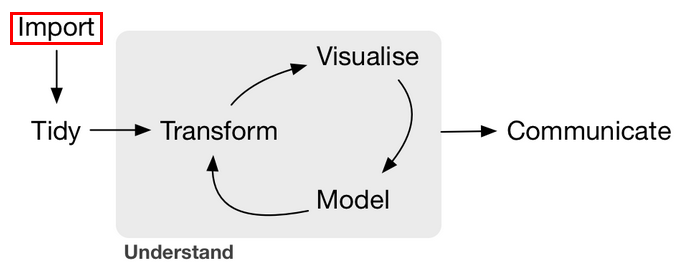
\includegraphics[width=0.75\textwidth]{../img/02_ciclo_1.png}
    \caption{Importación en el análisis de datos \textcite[Introducción]{grolemund2016r}.}
    \label{fig:ciclo1}
\end{figure}

Para aplicar las herramientas de R a nuestro trabajo, es necesario poder
importar nuestros datos a R. R tiene conectores ya implementados para
casi cualquier tipo y formato de datos. Entre los más comunes
están\footnote{La lista no pretende ser comprehensiva, sin embargo, se presentan algunos de los formatos de datos más comunes. De igual forma, se presentan algunas funciones que sirven para conectar \texttt{R} con datos que están guardados en un manejador de datos externo o en la nube. En caso de presentarse más de un método es porque aunque la recomendación de uso es la función en negritas, la otra opción es más antigua y muy utilizada.}:

\begin{longtable}[]{@{}lll@{}}
\toprule
Formato & Lectura & Escritura\tabularnewline
\midrule
\endhead
rds & \hyperref[rds]{base::readRDS} &
\hyperref[rds]{base::saveRDS}\tabularnewline
separado por * & \hyperref[separado-por]{utils::read.table};
\textbf{readr::read\_delim} &
\hyperref[separado-por]{utils::write.table};
\textbf{readr::write\_delim}\tabularnewline
csv & \hyperref[csv]{utils::read.csv}; \textbf{readr::read\_csv} &
\hyperref[csv]{utils::write.csv};
\textbf{readr::write\_csv}\tabularnewline
Microsoft Excel & \hyperref[microsoft-excel]{readxl::read\_excel} &
\hyperref[microsoft-excel]{xlsx::write.xlsx}\tabularnewline
dbf & \hyperref[dbf]{foreign::read.dbf} &
\hyperref[dbf]{foreign::write.dbf}\tabularnewline
IBM SPSS & \hyperref[ibm-spss]{haven::read\_sav} &
\hyperref[ibm-spss]{haven::write\_sav}\tabularnewline
Stata & \hyperref[stata]{haven::read\_dta} &
\hyperref[stata]{foreign::write.dta}\tabularnewline
SAS & \hyperref[sas]{haven::read\_sas} &
\hyperref[sas]{haven::write\_sas}\tabularnewline
Google spreadsheet &
\hyperref[google-spreadsheet]{googlesheets::gs\_read} &
\hyperref[google-spreadsheet]{googlesheets::gs\_new}\tabularnewline
Google bigquery & \hyperref[google-bigquery]{bigrquery::query\_exec}
&\tabularnewline
Heroku Postgres & \hyperref[heroku-postgres]{sql2df} &
\hyperref[heroku-postgres]{df2sql}\tabularnewline
rdata & \hyperref[rdata]{base::load} &
\hyperref[rdata]{base::save}\tabularnewline
\bottomrule
\end{longtable}

Los paquetes utilizados son (corre estos comandos en la consola):

\begin{Shaded}
\begin{Highlighting}[]
\KeywordTok{library}\NormalTok{(foreign)}
\KeywordTok{library}\NormalTok{(haven)}
\KeywordTok{library}\NormalTok{(readr)}
\KeywordTok{library}\NormalTok{(readxl)}
\KeywordTok{library}\NormalTok{(xlsx)}
\KeywordTok{library}\NormalTok{(googlesheets)}
\KeywordTok{library}\NormalTok{(bigrquery)}
\end{Highlighting}
\end{Shaded}

\begin{nota}[Importancia de rutas relativas]

Para leer un archivo, recordemos el comando \texttt{getwd()} para encontrar la carpeta
a la cual \texttt{R} esta dirigido en este momento. Una buena practica es considerar 
el directorio de trabajo como el lugar en donde esta guardado el archivo o \texttt{script} en el que se trabaja y ``moverse'' desde ahí hasta el archivo que se quiere leer.\\

Ya sea en escritura o en lectura, \texttt{R} buscará a partir del directorio
de trabajo (el que se despliega con \texttt{getwd()}) para buscar a partir 
de ahí el archivo por leer o para guardar el que se escribirá si se usan rutas
relativas.\\

En caso de usar rutas absolutas (a pesar de que esto \textbf{no} es una \textit{buena práctica}) se
hará lectura o escritura del archivo en el lugar especificado.
\end{nota}

\vspace{1cm}

\renewcommand\bcStyleTitre[1]{\large\textcolor{bbblack}{#1}}

\begin{bclogo}[
  couleur=llred,
  arrondi=0,
  logo=\bcstop,
  barre=none,
  noborder=true]{Ejercicios}
`R` tiene conexión con muchos de los formatos en los que se encuentran 
los datos. Veremos algunos de los mas relevantes.

El código en cada uno de los \texttt{chunks} (un chunk es el pedazo del documento
en donde hay código de \texttt{R}) está hecho para que puedas correrlo en la
consola (excepto cuando dice explícitamente \textit{do not run} (leyenda
comúnmente encontrada en los ejemplos de la documentación de las funciones. 
Con esto entenderás mejor el concepto de rutas relativas.
\end{bclogo}

\subsection{rds}\label{rds}

La extensión \texttt{rds} es de las más comúnmente utilizada en
\texttt{R}, por ejemplo, para guardar los datos para un paquete. Las
funciones pertenecen al \texttt{base} \parencite{rbase}. Permiten
guardar un solo objeto de \texttt{R} a un archivo y recuperarlo.

Para \textbf{escribirlos}

\begin{Shaded}
\begin{Highlighting}[]
\CommentTok{# Creamos un dataframe llamado misdatos}
\NormalTok{misdatos <-}\StringTok{ }\NormalTok{iris}
\CommentTok{# Los guardamos en comprimido}
\KeywordTok{saveRDS}\NormalTok{(misdatos, }\DataTypeTok{file =} \StringTok{"misdatos.rds"}\NormalTok{, }\DataTypeTok{ascii =} \OtherTok{FALSE}\NormalTok{, }\DataTypeTok{version =} \OtherTok{NULL}\NormalTok{,}
        \DataTypeTok{compress =} \OtherTok{TRUE}\NormalTok{, }\DataTypeTok{refhook =} \OtherTok{NULL}\NormalTok{)}
\end{Highlighting}
\end{Shaded}

Nota como si usas el comando \texttt{getwd()} y después vas a la ruta
indicada por medio del explorador de archivos, verás en esa carpeta el
archivo \texttt{misdatos.rds}.

Para \textbf{leerlos} usamos la ruta relativa. Dado que los guardamos en
el directorio de trabajo actual (Recuerda, se puede cambiar con el
comando \texttt{setwd}) entonces simplemente los llamamos:

\begin{Shaded}
\begin{Highlighting}[]
\NormalTok{misdatos <-}\StringTok{ }\KeywordTok{readRDS}\NormalTok{(}\StringTok{"misdatos.rds"}\NormalTok{)}
\CommentTok{# Los borramos}
\KeywordTok{file.remove}\NormalTok{(}\StringTok{"misdatos.rds"}\NormalTok{)}
\end{Highlighting}
\end{Shaded}

\subsection{separado por *}\label{separado-por}

Con esto nos referimos a la colección de archivos en texto plano, es
decir, \texttt{.txt}, \texttt{.tsv}, \texttt{.psv}, etcétera.

Para \textbf{escribirlos} el mas común es \texttt{write.table} del
paquete \texttt{utils} \parencite{utils}

\begin{Shaded}
\begin{Highlighting}[]
\CommentTok{# Do not run}
\KeywordTok{write.table}\NormalTok{(misdatos, }\DataTypeTok{file =} \StringTok{"~/misdatos.<extension>"}\NormalTok{, }\DataTypeTok{append =} \OtherTok{FALSE}
\NormalTok{, }\DataTypeTok{quote =} \OtherTok{TRUE}\NormalTok{, }\DataTypeTok{sep =} \StringTok{" "}\NormalTok{, }\DataTypeTok{eol =} \StringTok{"}\CharTok{\textbackslash{}n}\StringTok{"}\NormalTok{, }\DataTypeTok{na =} \StringTok{"NA"}\NormalTok{, }\DataTypeTok{dec =} \StringTok{"."}
\NormalTok{, }\DataTypeTok{row.names =} \OtherTok{TRUE}\NormalTok{, }\DataTypeTok{col.names =} \OtherTok{TRUE}
\NormalTok{, }\DataTypeTok{qmethod =} \KeywordTok{c}\NormalTok{(}\StringTok{"escape"}\NormalTok{, }\StringTok{"double"}\NormalTok{), }\DataTypeTok{fileEncoding =} \StringTok{""}\NormalTok{)}
\end{Highlighting}
\end{Shaded}

En el paquete \texttt{readr} se implementa también \texttt{write\_delim}

\begin{Shaded}
\begin{Highlighting}[]
\CommentTok{# Do not run}
\KeywordTok{write_delim}\NormalTok{(misdatos, }\DataTypeTok{path =} \StringTok{"~/misdatos.<extension>"}
\NormalTok{            , }\DataTypeTok{delim =} \StringTok{"}\CharTok{\textbackslash{}t}\StringTok{"}\NormalTok{, }\DataTypeTok{na =} \StringTok{"NA"}\NormalTok{, }\DataTypeTok{append =} \OtherTok{FALSE}\NormalTok{, }\DataTypeTok{col_names =} \OperatorTok{!}\NormalTok{append)}
\end{Highlighting}
\end{Shaded}

Escribamos ahora el \emph{dataframe} \texttt{misdatos} en \texttt{psv}:

\begin{Shaded}
\begin{Highlighting}[]
\KeywordTok{write_delim}\NormalTok{(misdatos, }\DataTypeTok{path =} \StringTok{"misdatos.psv"}\NormalTok{, }\DataTypeTok{delim =} \StringTok{"|"}\NormalTok{)}
\end{Highlighting}
\end{Shaded}

Para \textbf{leerlos} \texttt{read.table} del paquete \texttt{utils}
\parencite{utils} nos permite especificar casi cualquier particularidad
en un archivo de texto plano.

\begin{Shaded}
\begin{Highlighting}[]
\CommentTok{# Do not run}
\NormalTok{misdatos <-}\StringTok{ }\KeywordTok{read.table}\NormalTok{(}\StringTok{"~/misdatos.<extension>"}\NormalTok{, }\DataTypeTok{header =} \OtherTok{FALSE}
\NormalTok{                       , }\DataTypeTok{sep =} \StringTok{""}\NormalTok{, }\DataTypeTok{quote =} \StringTok{"}\CharTok{\textbackslash{}"}\StringTok{'"}\NormalTok{, }\DataTypeTok{dec =} \StringTok{"."}
\NormalTok{                       , }\DataTypeTok{numerals =} \KeywordTok{c}\NormalTok{(}\StringTok{"allow.loss"}\NormalTok{, }\StringTok{"warn.loss"}\NormalTok{, }\StringTok{"no.loss"}\NormalTok{)}
\NormalTok{                       , row.names, col.names, }\DataTypeTok{as.is =} \OperatorTok{!}\NormalTok{stringsAsFactors}
\NormalTok{                       , }\DataTypeTok{na.strings =} \StringTok{"NA"}\NormalTok{, }\DataTypeTok{colClasses =} \OtherTok{NA}\NormalTok{, }\DataTypeTok{nrows =} \OperatorTok{-}\DecValTok{1}
\NormalTok{                       , }\DataTypeTok{skip =} \DecValTok{0}\NormalTok{, }\DataTypeTok{check.names =} \OtherTok{TRUE}
\NormalTok{                       , }\DataTypeTok{fill =} \OperatorTok{!}\NormalTok{blank.lines.skip, }\DataTypeTok{strip.white =} \OtherTok{FALSE}
\NormalTok{                       , }\DataTypeTok{blank.lines.skip =} \OtherTok{TRUE}\NormalTok{, }\DataTypeTok{comment.char =} \StringTok{"#"}
\NormalTok{                       , }\DataTypeTok{allowEscapes =} \OtherTok{FALSE}\NormalTok{, }\DataTypeTok{flush =} \OtherTok{FALSE}
\NormalTok{                       , }\DataTypeTok{stringsAsFactors =} \KeywordTok{default.stringsAsFactors}\NormalTok{()}
\NormalTok{                       , }\DataTypeTok{fileEncoding =} \StringTok{""}\NormalTok{, }\DataTypeTok{encoding =} \StringTok{"unknown"}\NormalTok{, text}
\NormalTok{                       , }\DataTypeTok{skipNul =} \OtherTok{FALSE}\NormalTok{)}
\end{Highlighting}
\end{Shaded}

La función \texttt{read\_delim} del paquete \texttt{readr}
\parencite{readr} lee los datos más eficientemente a un objeto de clase
\texttt{tibble}.

\begin{Shaded}
\begin{Highlighting}[]
\CommentTok{# Do not run}
\NormalTok{misdatos <-}\StringTok{ }\KeywordTok{read_delim}\NormalTok{(}\DataTypeTok{file =} \StringTok{"~/misdatos.<extension>"}\NormalTok{, delim}
\NormalTok{                       , }\DataTypeTok{quote =} \StringTok{"}\CharTok{\textbackslash{}"}\StringTok{"}\NormalTok{, }\DataTypeTok{escape_backslash =} \OtherTok{FALSE}
\NormalTok{                       , }\DataTypeTok{escape_double =} \OtherTok{TRUE}\NormalTok{, }\DataTypeTok{col_names =} \OtherTok{TRUE}
\NormalTok{                       , }\DataTypeTok{col_types =} \OtherTok{NULL}\NormalTok{, }\DataTypeTok{locale =} \KeywordTok{default_locale}\NormalTok{()}
\NormalTok{                       , }\DataTypeTok{na =} \KeywordTok{c}\NormalTok{(}\StringTok{""}\NormalTok{, }\StringTok{"NA"}\NormalTok{), }\DataTypeTok{quoted_na =} \OtherTok{TRUE}\NormalTok{, }\DataTypeTok{comment =} \StringTok{""}
\NormalTok{                       , }\DataTypeTok{trim_ws =} \OtherTok{FALSE}\NormalTok{, }\DataTypeTok{skip =} \DecValTok{0}\NormalTok{, }\DataTypeTok{n_max =} \OtherTok{Inf}
\NormalTok{                       , }\DataTypeTok{guess_max =} \KeywordTok{min}\NormalTok{(}\DecValTok{1000}\NormalTok{, n_max)}
\NormalTok{                       , }\DataTypeTok{progress =} \KeywordTok{interactive}\NormalTok{())}
\end{Highlighting}
\end{Shaded}

Leemos el archivo \texttt{.psv} que creamos antes:

\begin{Shaded}
\begin{Highlighting}[]
\NormalTok{misdatos <-}\StringTok{ }\KeywordTok{read_delim}\NormalTok{(}\DataTypeTok{file =} \StringTok{"misdatos.psv"}\NormalTok{, }\DataTypeTok{delim =} \StringTok{"|"}\NormalTok{)}
\CommentTok{# Los borramos}
\KeywordTok{file.remove}\NormalTok{(}\StringTok{"misdatos.psv"}\NormalTok{)}
\end{Highlighting}
\end{Shaded}

\subsection{csv (archivo separado por
comas)}\label{csv-archivo-separado-por-comas}

Este es un caso particular de archivos de texto en el que se separan por
comas. Como es muy utilizado, generalmente se hacen funciones donde ya
se especifica el delimitador. Guardaremos el \emph{data frame}
\texttt{misdatos} en el directorio ``arriba'' de la ruta que se muestra
usando \texttt{getwd}. Esto lo podemos hacer anteponiendo al nombre del
archivo con \texttt{../}.

Para \textbf{escribirlos}

\begin{Shaded}
\begin{Highlighting}[]
\CommentTok{# utils }
\KeywordTok{write.csv}\NormalTok{(misdatos, }\DataTypeTok{file =} \StringTok{"../misdatos.csv"}\NormalTok{, }\DataTypeTok{row.names =}\NormalTok{ F)}
\CommentTok{# readr}
\KeywordTok{write_csv}\NormalTok{(misdatos, }\DataTypeTok{path =} \StringTok{"../misdatos.csv"}\NormalTok{, }\DataTypeTok{na =} \StringTok{"NA"}\NormalTok{, }\DataTypeTok{append =} \OtherTok{FALSE}\NormalTok{)}
\end{Highlighting}
\end{Shaded}

Observa en el explorador de archivos en dónde es que se guardó el
archivo \texttt{misdatos.csv}.

Para \textbf{leerlos}, seguimos usando rutas relativas.

\begin{Shaded}
\begin{Highlighting}[]
\CommentTok{# utils - como data.frame}
\NormalTok{misdatos <-}\StringTok{ }\KeywordTok{read.table}\NormalTok{(}\StringTok{"../misdatos.csv"}\NormalTok{, }\DataTypeTok{header=}\OtherTok{TRUE}\NormalTok{,}
   \DataTypeTok{sep=}\StringTok{","}\NormalTok{)}

\NormalTok{misdatos <-}\StringTok{ }\KeywordTok{read.csv}\NormalTok{(}\StringTok{"../misdatos.csv"}\NormalTok{)}

\CommentTok{# readr - como tibble}
\NormalTok{misdatos <-}\StringTok{ }\KeywordTok{read_csv}\NormalTok{(}\StringTok{"../misdatos.csv"}\NormalTok{)}

\CommentTok{# Lo borro}
\KeywordTok{file.remove}\NormalTok{(}\StringTok{"../misdatos.csv"}\NormalTok{)}
\end{Highlighting}
\end{Shaded}

\subsection{Microsoft Excel}\label{microsoft-excel}

Para \textbf{escribirlos} dentro del paquete \texttt{xlsx} usamos la
función \texttt{write.xlsx}

\begin{Shaded}
\begin{Highlighting}[]
\NormalTok{misdatos <-}\StringTok{ }\NormalTok{iris}
\KeywordTok{write.xlsx}\NormalTok{(misdatos, }\StringTok{"misdatos.xlsx"}\NormalTok{, }\DataTypeTok{row.names =}\NormalTok{ F)}
\end{Highlighting}
\end{Shaded}

Para \textbf{leerlos} dentro del paquete \texttt{readxl} se encuentra la
función \texttt{read\_excel} que es muy útil en este caso.

\begin{Shaded}
\begin{Highlighting}[]
\NormalTok{misdatos <-}\StringTok{ }\KeywordTok{read_excel}\NormalTok{(}\StringTok{"misdatos.xlsx"}\NormalTok{, }\DataTypeTok{sheet =} \DecValTok{1}\NormalTok{, }\DataTypeTok{col_names =} \OtherTok{TRUE}\NormalTok{, }
\DataTypeTok{col_types =} \OtherTok{NULL}\NormalTok{, }\DataTypeTok{na =} \StringTok{""}\NormalTok{, }\DataTypeTok{skip =} \DecValTok{0}\NormalTok{)}

\CommentTok{# Lo borro}
\KeywordTok{file.remove}\NormalTok{(}\StringTok{"misdatos.xlsx"}\NormalTok{)}
\end{Highlighting}
\end{Shaded}

\subsection{dbf}\label{dbf}

Extensión que representa un archivo de una base de datos (\emph{database
file}).

Para \textbf{escribirlos}:

\begin{Shaded}
\begin{Highlighting}[]
\KeywordTok{write.dbf}\NormalTok{(}\KeywordTok{as.data.frame}\NormalTok{(misdatos), }\StringTok{"misdatos.dbf"}\NormalTok{)}
\end{Highlighting}
\end{Shaded}

Nota cómo tuvimos que coercionar el objeto a \emph{data frame}. Como en
el ejemplo anterior leímos un \emph{tibble} y el paquete
\texttt{foreign} es más viejo (y no conoce los \emph{tibbles}) entonces
le mandamos un objeto que si conoce.

Veremos más adelante la ventaja de usar \emph{tibbles} aún cuando de vez
en cuando se tienen problemas de compatibilidad.

Para \textbf{leerlos}:

\begin{Shaded}
\begin{Highlighting}[]
\NormalTok{misdatos <-}\StringTok{ }\KeywordTok{read.dbf}\NormalTok{(}\StringTok{"misdatos.dbf"}\NormalTok{)}
\CommentTok{# Lo borro}
\KeywordTok{file.remove}\NormalTok{(}\StringTok{"misdatos.dbf"}\NormalTok{)}
\end{Highlighting}
\end{Shaded}

\subsection{IBM SPSS}\label{ibm-spss}

SPSS puede guardar los datos agregando etiquetas y otros metadatos. Para
evitar retrabajo, puede leerse directamente a \texttt{R}.

Para \textbf{escribirlos}

\begin{Shaded}
\begin{Highlighting}[]
\CommentTok{# haven}
\KeywordTok{write_sav}\NormalTok{(}\DataTypeTok{data =}\NormalTok{ misdatos, }\DataTypeTok{path =} \StringTok{"misdatos.sav"}\NormalTok{)}
\end{Highlighting}
\end{Shaded}

Para \textbf{leerlos}

\begin{Shaded}
\begin{Highlighting}[]
\CommentTok{# haven - como tibble}
\NormalTok{misdatos <-}\StringTok{ }\KeywordTok{read_sav}\NormalTok{(}\DataTypeTok{file =} \StringTok{"misdatos.sav"}\NormalTok{, }\DataTypeTok{user_na =} \OtherTok{FALSE}\NormalTok{)}

\CommentTok{# Lo borro}
\KeywordTok{file.remove}\NormalTok{(}\StringTok{"misdatos.sav"}\NormalTok{)}
\end{Highlighting}
\end{Shaded}

\subsection{Stata}\label{stata}

\begin{curiosidad}[HOME DIRECTORY]
El directorio (carpeta) \textit{home} es muy utilizado. Normalmente, se le 
denota como $\thicksim$ y es en donde un sistema operativo guarda los 
archivos del usuario que se encuentra en sesión. Dependiendo del sistema
operativo que utilices, encontrarás este directorio en una ruta específica.\\

En Microsoft Windows Vista 7, 8 y 10 lo encuentras en \texttt{<root>$\backslash$Users$\backslash$<username>}.\\

En Linux lo encuentras en \texttt{$/$home$/$<username>}.\\

En Mac OS X lo encuentras en \texttt{$/$Users$/$<username>}.
\end{curiosidad}

Para \textbf{escribirlos} en \texttt{Stata} primero tenemos que cambiar
los nombres de las variables en el \emph{data frame} pues \texttt{Stata}
no admite puntos en los nombres:

\begin{Shaded}
\begin{Highlighting}[]
\KeywordTok{names}\NormalTok{(misdatos) <-}\StringTok{ }\KeywordTok{tolower}\NormalTok{(}\KeywordTok{gsub}\NormalTok{(}\StringTok{"}\CharTok{\textbackslash{}\textbackslash{}}\StringTok{."}\NormalTok{, }\StringTok{"_"}\NormalTok{, }\KeywordTok{names}\NormalTok{(misdatos)))}
\CommentTok{# foreign}
\KeywordTok{write.dta}\NormalTok{(}\DataTypeTok{data =}\NormalTok{ misdatos, }\DataTypeTok{file =} \StringTok{"~/misdatos.dta"}\NormalTok{, }\DataTypeTok{version =} \DecValTok{12}\NormalTok{)}
\end{Highlighting}
\end{Shaded}

Para \textbf{leerlos}

\begin{Shaded}
\begin{Highlighting}[]
\CommentTok{# haven - como tibble}
\NormalTok{misdatos <-}\StringTok{ }\KeywordTok{read_dta}\NormalTok{(}\DataTypeTok{file =} \StringTok{"~/misdatos.dta"}\NormalTok{, }\DataTypeTok{encoding =} \OtherTok{NULL}\NormalTok{)}

\CommentTok{# Lo borramos}
\KeywordTok{file.remove}\NormalTok{(}\StringTok{"~/misdatos.dta"}\NormalTok{)}
\end{Highlighting}
\end{Shaded}

\subsection{SAS}\label{sas}

Para usar el paquete \texttt{haven} en este caso ejemplificaremos la
creación de un directorio de archivos en tu computadora desde
\texttt{R}:

\begin{Shaded}
\begin{Highlighting}[]
\CommentTok{# Creamos un directorio llamado datos}
\KeywordTok{dir.create}\NormalTok{(}\StringTok{"datos_sas"}\NormalTok{)}
\end{Highlighting}
\end{Shaded}

Observa como, en el directorio que se despliega con \texttt{getwd}
encuentras ahora una carpeta llamada \texttt{datos\_sas}. Creamos ahí un
archivo con la función \texttt{write\_sas} de \texttt{haven}. Nota que,
para \textbf{escribirlos}, también debemos asegurarnos que los nombres
de variables estén compuestos por letras, números o guiones bajos:

\begin{Shaded}
\begin{Highlighting}[]
\NormalTok{misdatos <-}\StringTok{ }\NormalTok{iris}
\KeywordTok{names}\NormalTok{(misdatos) <-}\StringTok{ }\KeywordTok{tolower}\NormalTok{(}\KeywordTok{gsub}\NormalTok{(}\StringTok{"}\CharTok{\textbackslash{}\textbackslash{}}\StringTok{."}\NormalTok{, }\StringTok{"_"}\NormalTok{, }\KeywordTok{names}\NormalTok{(misdatos)))}
\CommentTok{# haven}
\KeywordTok{write_sas}\NormalTok{(}\DataTypeTok{data =}\NormalTok{ misdatos, }\DataTypeTok{path =} \StringTok{"datos_sas/misdatos.sas7bdat"}\NormalTok{)}
\end{Highlighting}
\end{Shaded}

Para leerlos, utilizamos \texttt{read\_sas} del paquete \texttt{haven}:

\begin{Shaded}
\begin{Highlighting}[]
\CommentTok{# haven - como tibble}
\NormalTok{misdatos <-}\StringTok{ }\KeywordTok{read_sas}\NormalTok{(}\StringTok{"datos_sas/misdatos.sas7bdat"}
\NormalTok{                     , }\DataTypeTok{catalog_file =} \OtherTok{NULL}\NormalTok{, }\DataTypeTok{encoding =} \OtherTok{NULL}\NormalTok{)}
\end{Highlighting}
\end{Shaded}

Observa desde el explorador de archivos, cómo se creó el archivo dentro
del directorio \texttt{datos\_sas/}. También desde \texttt{R} podemos
borrar el directorio:

\begin{Shaded}
\begin{Highlighting}[]
\KeywordTok{unlink}\NormalTok{(}\StringTok{"datos_sas"}\NormalTok{, }\DataTypeTok{recursive =}\NormalTok{ T, }\DataTypeTok{force =} \OtherTok{FALSE}\NormalTok{)}
\end{Highlighting}
\end{Shaded}

La bandera \texttt{recursive} le dice al sistema que borre todo lo
contenido en esa carpeta.

\subsection{Google Spreadsheet}\label{google-spreadsheet}

Para hacer este ejercicio, debes tener una cuenta de \texttt{gmail}.

Primero, debe realizarse la autenticación. Esto lo puedes hacer en
cualquier sesión interactiva utilizando alguna función del paquete
\texttt{googlesheets}

\begin{Shaded}
\begin{Highlighting}[]
\KeywordTok{gs_ls}\NormalTok{()}
\end{Highlighting}
\end{Shaded}

En la consola de \texttt{R} te aparece:

\begin{figure}[H]
\centering
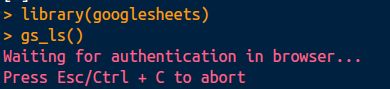
\includegraphics[width=0.3\textwidth]{../img/gs_oauth1.png}
\end{figure}

Se abrirá una ventana del explorador y deberás introducir tus
credenciales de tu cuenta de \texttt{gmail}

\begin{figure}[H]
\centering
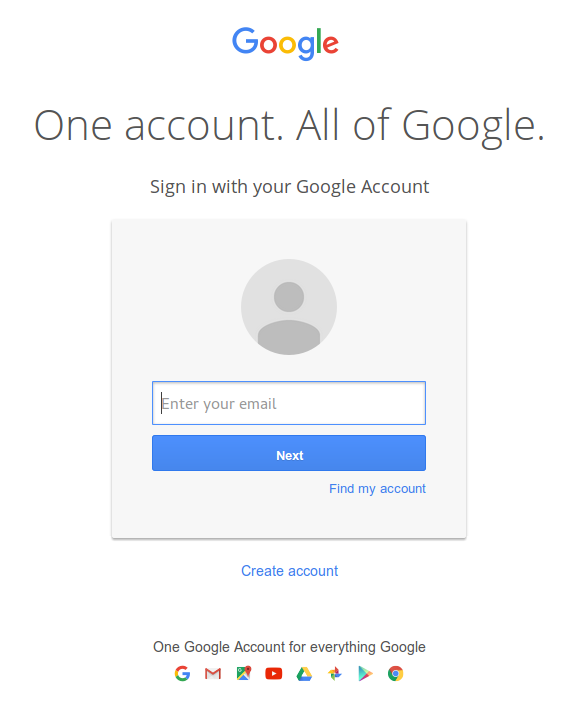
\includegraphics[width=0.5\textwidth]{../img/gs_oauth2.png}
\end{figure}

Después de poner tus credenciales, te aparecerá un mensaje pidiendo
acceso a tus datos en \texttt{drive}:

\begin{figure}[H]
\centering
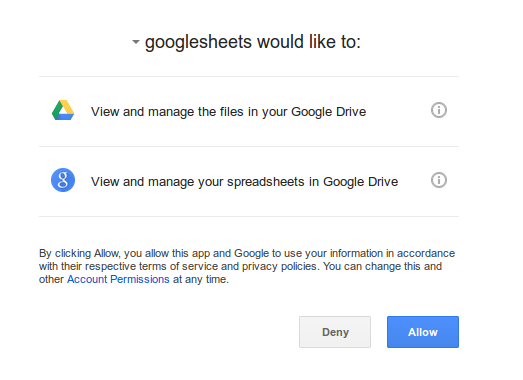
\includegraphics[width=0.5\textwidth]{../img/gs_oauth3.png}
\end{figure}

Al aceptar darle acceso, recibirás un mensaje parecido a
\emph{Authentication complete. Please close this page and return to R.}

Ahora verás en la consola de R un listado de las
\texttt{google\ spreadsheets} en tu cuenta de \texttt{gmail}.

Ahora, vamos a \textbf{escribir} una nueva hoja en tu cuenta.

\begin{Shaded}
\begin{Highlighting}[]
\KeywordTok{gs_new}\NormalTok{(}\StringTok{"misdatos"}\NormalTok{, }\DataTypeTok{ws_title =} \StringTok{"mihoja"}\NormalTok{, }\DataTypeTok{input =} \KeywordTok{head}\NormalTok{(iris)}
\NormalTok{       , }\DataTypeTok{trim =} \OtherTok{TRUE}\NormalTok{, }\DataTypeTok{verbose =} \OtherTok{FALSE}\NormalTok{)}
\end{Highlighting}
\end{Shaded}

Si vas a tu google drive, deberás ver que se creó un nuevo elemento que
se ve así:

\begin{figure}[H]
\centering
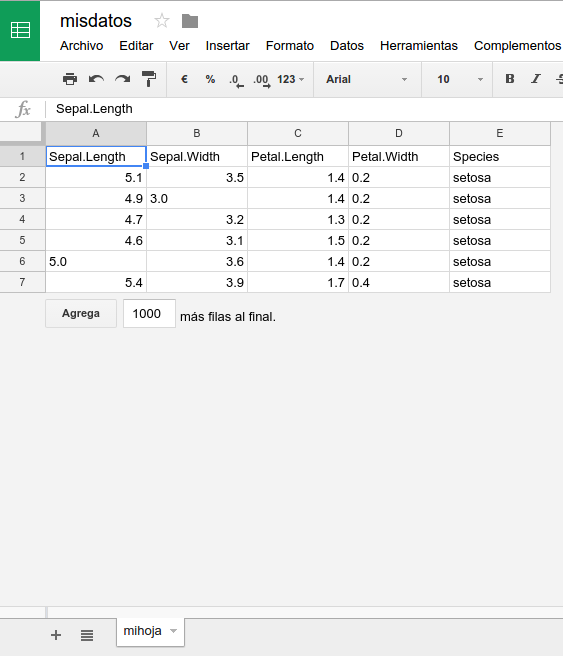
\includegraphics[width=0.5\textwidth]{../img/gs_nuevo.png}
\end{figure}

De igual forma, puedes ahora \textbf{leer} los datos de cualquier
\texttt{google\ spreadsheet} que tengas en tu cuenta.

\begin{Shaded}
\begin{Highlighting}[]
\NormalTok{misdatos <-}\StringTok{ }\KeywordTok{gs_read}\NormalTok{(}\KeywordTok{gs_title}\NormalTok{(}\StringTok{"misdatos"}\NormalTok{), }\DataTypeTok{ws =} \StringTok{"mihoja"}\NormalTok{)}
\CommentTok{# La borro}
\KeywordTok{gs_delete}\NormalTok{(}\KeywordTok{gs_title}\NormalTok{(}\StringTok{"misdatos"}\NormalTok{))}
\end{Highlighting}
\end{Shaded}

\subsection{Google bigquery}\label{google-bigquery}

\texttt{Google\ bigquery} es un \emph{data warehouse} que permite
guardar grandes bases de datos. Al contratar el servicio,
\texttt{google} se encarga del \emph{hardware} y la infraestructura
necesaria para que su procesamiento sea rápido
\parencite{whatisbigquery}.

Para guardar tus datos en \texttt{bigquery} debes crear un proyecto en
\href{https://console.developers.google.com/apis/library}{la consola de
desarrolladores}.

Existen varias bases de dato públicas disponibles. Para poder
utilizarlas, necesitas tener una cuenta. Puedes empezar una prueba
gratis en \href{https://cloud.google.com/free-trial/}{la página de
google cloud platform.} Verás una pantalla como esta:

\begin{figure}[H]
\centering
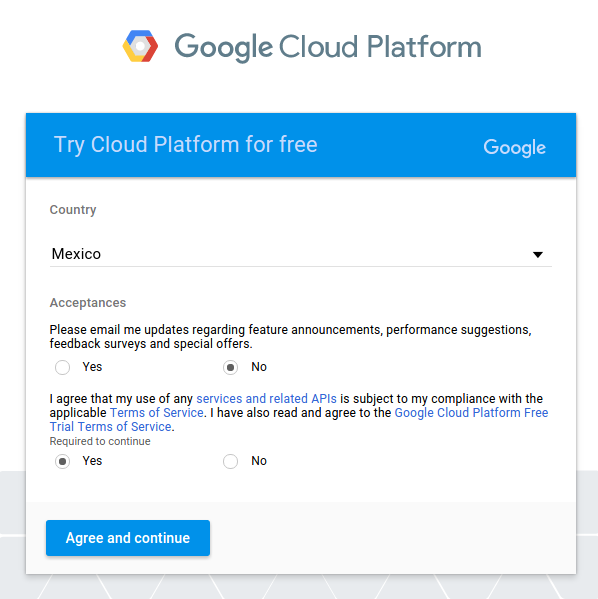
\includegraphics[width=0.5\textwidth]{../img/bq1.png}
\end{figure}

Sigue las instrucciones y eventualmente llegarás a una pantalla como
esta

\begin{figure}[H]
\centering
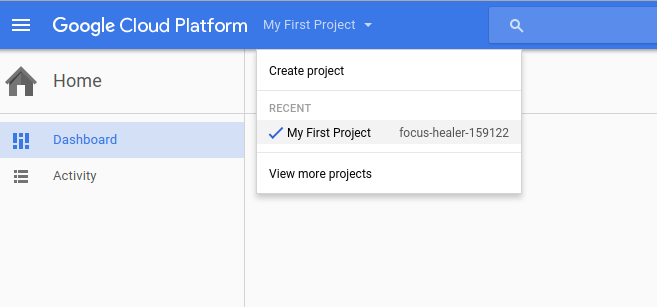
\includegraphics[width=0.5\textwidth]{../img/bq2.png}
\end{figure}

Copia el identificador de tu proyecto para que puedas realizar
\texttt{queries} (llamadas a las bases de datos).

Leemos la base de datos pública de natalidad en Estados Unidos.

\begin{Shaded}
\begin{Highlighting}[]
\NormalTok{project <-}\StringTok{ "focus-healer-159122"} \CommentTok{# pon tu projectID aquí}
 
\NormalTok{sql <-}\StringTok{ 'SELECT year, count(*) as babies, avg(mother_age) as mother_age_avg}
\StringTok{FROM[publicdata:samples.natality] }
\StringTok{WHERE year > 1980 and year < 2006}
\StringTok{group by year;'}
 
\NormalTok{data <-}\StringTok{ }\KeywordTok{query_exec}\NormalTok{(}\DataTypeTok{query =}\NormalTok{ sql, }\DataTypeTok{project =}\NormalTok{ project)}
\end{Highlighting}
\end{Shaded}

Nota como la tabla cuenta con aproximadamente. 140 millones de registros
y se obtiene el detalle en segundos.

\subsection{Heroku Postgres}\label{heroku-postgres}

\texttt{R} no es un manejador de base de datos y, por ende, no es un
lenguaje que permite trabajar con una gran cantidad de datos. \texttt{R}
guarda los objetos utilizando la memoria virtual de la computadora,
i.e.~la RAM, misma que depende de varios elementos (incluido el sistema
operativo) y que limita los datos que podrán ser procesados.

Cuando necesitamos conocer el tamaño de los datos que están en el
ambiente de trabajo, puede utilizarse el paquete \texttt{pryr}
\parencite[][sección ``the role of physical memory'']{pryr}.

\begin{Shaded}
\begin{Highlighting}[]
\KeywordTok{rm}\NormalTok{(}\DataTypeTok{list =} \KeywordTok{ls}\NormalTok{()) }\CommentTok{# borramos los objetos del ambiente}
\CommentTok{# Cargamos datos al ambiente}
\NormalTok{flights <-}\StringTok{ }\KeywordTok{read_csv}\NormalTok{(}\StringTok{"data/flights.csv"}\NormalTok{)}
\NormalTok{airports <-}\StringTok{ }\KeywordTok{read_csv}\NormalTok{(}\StringTok{"data/airports.csv"}\NormalTok{)}
\NormalTok{planes <-}\StringTok{ }\KeywordTok{read_csv}\NormalTok{(}\StringTok{"data/planes.csv"}\NormalTok{)}
\KeywordTok{ls}\NormalTok{() }\CommentTok{# mostramos los objetos en el ambiente}

\KeywordTok{library}\NormalTok{(pryr) }\CommentTok{# Cargamos el paquete pryr}
\KeywordTok{mem_used}\NormalTok{() }\CommentTok{# memoria utilizada}

\KeywordTok{object_size}\NormalTok{(flights, }\DataTypeTok{units =} \StringTok{"Mb"}\NormalTok{) }\CommentTok{# Obtenemos el tamaño de un objeto}
\KeywordTok{sapply}\NormalTok{(}\KeywordTok{ls}\NormalTok{(), }\ControlFlowTok{function}\NormalTok{(x) }\KeywordTok{object_size}\NormalTok{(}\KeywordTok{get}\NormalTok{(x))) }\CommentTok{# de todos en el ambiente}
\end{Highlighting}
\end{Shaded}

Las estrategias en memoria se revisaron brevemente en el apartado XXX,
en este caso, es pertinente mencionar las estrategias fuera de memoria
(\emph{out of memory}).

Es posible explorar un conjunto de datos sin necesidad de cargarlos en
\texttt{R} pero utilizando comandos de \texttt{R} y trabajando desde un
script de \texttt{R}, permitiendo que herramientas más eficientes (y
apropiadas) para el trabajo de grandes volúmenes de datos realicen el
procesamiento de los mismos.

Los sistemas gestores de base de datos están optimizados para almacenar
y buscar en grandes volúmenes de datos en forma más eficiente que
\texttt{R}. Algunos ejemplos populares son Oracle y PostgreSQL
\parencite[][sección ``working with large datasets'']{peng2016m}. Hay
múltiples paquetes que permiten establecer una conexión con estos
sistemas desde una sesión de \texttt{R}.

Los paquetes \texttt{DBI} y \texttt{Postgresql} permiten realizar esta
tarea. Debido a que requieren credenciales se muestra una función para
leer datos desde \texttt{PostgreSQL} y escribirlos sin necesidad de
poner las credenciales dentro del mismo script.

Para que funcionen apropiadamente, es necesario poner en el directorio
de trabajo un archivo llamado \texttt{parametros.yaml} en donde se
escriben las credenciales para Postgres:

\begin{verbatim}
host : localhost
db : postgres
username : usr
password : password
\end{verbatim}

Nota: el salto de línea en la última línea es importante.

Para leer datos, creamos una función a la que podemos enviarle una
cadena de comandos en SQL.

\begin{Shaded}
\begin{Highlighting}[]
\NormalTok{sql2df <-}\StringTok{ }\ControlFlowTok{function}\NormalTok{(sql.file, }\DataTypeTok{df.file =} \StringTok{""}\NormalTok{) \{}
  \KeywordTok{require}\NormalTok{(DBI)}
  \KeywordTok{require}\NormalTok{(futile.logger)}
  \KeywordTok{require}\NormalTok{(yaml)}
  \KeywordTok{require}\NormalTok{(RPostgreSQL)}
  
  \ControlFlowTok{if}\NormalTok{(}\OperatorTok{!}\KeywordTok{file.exists}\NormalTok{(df.file)) \{}
    \ControlFlowTok{if}\NormalTok{(}\KeywordTok{file.exists}\NormalTok{(}\StringTok{"./parametros.yaml"}\NormalTok{)) \{}
\NormalTok{      x <-}\StringTok{ }\NormalTok{yaml}\OperatorTok{::}\KeywordTok{yaml.load_file}\NormalTok{(}\StringTok{"./parametros.yaml"}\NormalTok{)}
\NormalTok{    \} }\ControlFlowTok{else}\NormalTok{ \{}
\NormalTok{      x <-}\StringTok{ }\NormalTok{yaml}\OperatorTok{::}\KeywordTok{yaml.load_file}\NormalTok{(}\StringTok{"../parametros.yaml"}\NormalTok{)}
\NormalTok{    \}}
    
    \CommentTok{# Creamos la conexión a la base de datos}
\NormalTok{    futile.logger}\OperatorTok{::}\KeywordTok{flog.info}\NormalTok{(}\StringTok{"Conectando a la base de datos"}\NormalTok{)}
    
\NormalTok{    con <-}\StringTok{ }\KeywordTok{dbConnect}\NormalTok{(RPostgreSQL}\OperatorTok{::}\KeywordTok{PostgreSQL}\NormalTok{(), }\DataTypeTok{dbname =}\NormalTok{ x}\OperatorTok{$}\NormalTok{db, }
                     \DataTypeTok{host =}\NormalTok{ x}\OperatorTok{$}\NormalTok{host, }
                     \DataTypeTok{port =} \DecValTok{5432}\NormalTok{, }
                     \DataTypeTok{user =}\NormalTok{ x}\OperatorTok{$}\NormalTok{username,}
                     \DataTypeTok{password =}\NormalTok{ x}\OperatorTok{$}\NormalTok{password)}
    
\NormalTok{    futile.logger}\OperatorTok{::}\KeywordTok{flog.info}\NormalTok{(}\StringTok{"Conectado a %s, como %s"}\NormalTok{, x}\OperatorTok{$}\NormalTok{host, x}\OperatorTok{$}\NormalTok{username)}
    
    \CommentTok{# Leemos el query}
\NormalTok{    sql <-}\StringTok{ }\KeywordTok{paste}\NormalTok{(}\KeywordTok{readLines}\NormalTok{(sql.file,}\DataTypeTok{encoding=}\StringTok{"UTF-8"}\NormalTok{)}
\NormalTok{                 , }\DataTypeTok{sep=}\StringTok{" "}\NormalTok{, }\DataTypeTok{collapse=}\StringTok{" "}\NormalTok{)}
    
    \KeywordTok{tryCatch}\NormalTok{( \{}
\NormalTok{      futile.logger}\OperatorTok{::}\KeywordTok{flog.info}\NormalTok{(}\StringTok{"Ejecutando el query"}\NormalTok{)}
      \CommentTok{# Creamos el query}
\NormalTok{      rs <-}\StringTok{ }\NormalTok{RPostgreSQL}\OperatorTok{::}\KeywordTok{dbSendQuery}\NormalTok{(con, sql)}
\NormalTok{      futile.logger}\OperatorTok{::}\KeywordTok{flog.info}\NormalTok{(}\StringTok{"Obteniendo los datos"}\NormalTok{)}
      \CommentTok{# Obtenemos los datos}
\NormalTok{      df <-}\StringTok{ }\NormalTok{DBI}\OperatorTok{::}\KeywordTok{dbFetch}\NormalTok{(rs)}
      \CommentTok{# Liberamos el ResultSet}
\NormalTok{      futile.logger}\OperatorTok{::}\KeywordTok{flog.info}\NormalTok{(}\StringTok{"Limpiando el result set"}\NormalTok{)}
\NormalTok{      RPostgreSQL}\OperatorTok{::}\KeywordTok{dbClearResult}\NormalTok{(rs)}
\NormalTok{    \}, }\DataTypeTok{finally=}\NormalTok{RPostgreSQL}\OperatorTok{::}\KeywordTok{dbDisconnect}\NormalTok{(con) }\CommentTok{# Nos desconectamos de la BD}
\NormalTok{    )}
    
    \ControlFlowTok{if}\NormalTok{(df.file }\OperatorTok{!=}\StringTok{ ""}\NormalTok{)\{ }
      \KeywordTok{saveRDS}\NormalTok{(}\DataTypeTok{object=}\NormalTok{df, }\DataTypeTok{file=}\NormalTok{df.file)  }
\NormalTok{    \}}
\NormalTok{  \} }\ControlFlowTok{else}\NormalTok{ \{}
\NormalTok{    df <-}\StringTok{ }\KeywordTok{readRDS}\NormalTok{(df.file)}
\NormalTok{  \}}
  
  \KeywordTok{return}\NormalTok{(df)}
\NormalTok{\}}
\end{Highlighting}
\end{Shaded}

La función
\texttt{sql2df}\footnote{Función adaptada de notas de Adolfo de Únanue.}
recibe como parámetro, como cadena, la ruta hacia un archivo de
extensión \texttt{.sql} con los comandos a ejecutar en el manejador de
base de datos. Éste puede verse, por ejemplo, como:

\begin{verbatim}
select * 
from information_schema.tables 
where table_schema = 'information_schema';
\end{verbatim}

Guardamos ésta en el archivo \texttt{sql/ejemplo.sql} la cláusula de
arriba. Después, llamamos a la función.

\begin{Shaded}
\begin{Highlighting}[]
\NormalTok{datos <-}\StringTok{ }\KeywordTok{sql2df}\NormalTok{(}\StringTok{"sql/ejemplo.sql"}\NormalTok{, }\DataTypeTok{df.file =} \StringTok{"ejemplo.rds"}\NormalTok{)}
\KeywordTok{head}\NormalTok{(datos)}
\end{Highlighting}
\end{Shaded}

Con el parámetro \texttt{df.file} es posible especificar una ruta para
que se guarde una copia local del resultado de los datos. Esto es útil
cuando se está trabajando con los datos, de forma que sea más rápido el
trabajo con los mismos.

Para escribir datos, podemos utilizar la función siguiente:

\begin{Shaded}
\begin{Highlighting}[]
\NormalTok{df2sql <-}\StringTok{ }\ControlFlowTok{function}\NormalTok{(data.frame, df.schema.name, df.table.name, }\DataTypeTok{owner.to =} \OtherTok{NA}\NormalTok{) \{}
  \KeywordTok{require}\NormalTok{(DBI)}
  \KeywordTok{require}\NormalTok{(futile.logger)}
  \KeywordTok{require}\NormalTok{(yaml)}
  \KeywordTok{require}\NormalTok{(RPostgreSQL)}
\NormalTok{  data.frame <-}\StringTok{ }\KeywordTok{data.frame}\NormalTok{(data.frame)}
  \CommentTok{# Normalizamos nombres}
  \KeywordTok{names}\NormalTok{(data.frame) <-}\StringTok{ }\KeywordTok{normalizarNombres}\NormalTok{(}\KeywordTok{names}\NormalTok{(data.frame))}
  
  \ControlFlowTok{if}\NormalTok{(}\KeywordTok{file.exists}\NormalTok{(}\StringTok{"./parametros.yaml"}\NormalTok{)) \{}
\NormalTok{    x <-}\StringTok{ }\NormalTok{yaml}\OperatorTok{::}\KeywordTok{yaml.load_file}\NormalTok{(}\StringTok{"./parametros.yaml"}\NormalTok{)}
\NormalTok{  \} }\ControlFlowTok{else}\NormalTok{ \{}
\NormalTok{    x <-}\StringTok{ }\NormalTok{yaml}\OperatorTok{::}\KeywordTok{yaml.load_file}\NormalTok{(}\StringTok{"../parametros.yaml"}\NormalTok{)}
\NormalTok{  \}}
   
  \CommentTok{# Creamos la conexión a la base de datos}
\NormalTok{  futile.logger}\OperatorTok{::}\KeywordTok{flog.info}\NormalTok{(}\StringTok{"Conectando a la base de datos"}\NormalTok{)}
    
\NormalTok{  con <-}\StringTok{ }\KeywordTok{dbConnect}\NormalTok{(RPostgreSQL}\OperatorTok{::}\KeywordTok{PostgreSQL}\NormalTok{(), }\DataTypeTok{dbname =}\NormalTok{ x}\OperatorTok{$}\NormalTok{db, }
                     \DataTypeTok{host =}\NormalTok{ x}\OperatorTok{$}\NormalTok{host, }
                     \DataTypeTok{port =} \DecValTok{5432}\NormalTok{, }
                     \DataTypeTok{user =}\NormalTok{ x}\OperatorTok{$}\NormalTok{username,}
                     \DataTypeTok{password =}\NormalTok{ x}\OperatorTok{$}\NormalTok{password)}
\NormalTok{  futile.logger}\OperatorTok{::}\KeywordTok{flog.info}\NormalTok{(}\StringTok{"Conectado a %s, como %s"}
\NormalTok{                           , x}\OperatorTok{$}\NormalTok{host, x}\OperatorTok{$}\NormalTok{username)}
  
  \KeywordTok{tryCatch}\NormalTok{( \{}
    \KeywordTok{flog.info}\NormalTok{(}\StringTok{"Ejecutando la escritura de tabla %s en el esquema %s"}
\NormalTok{              , df.table.name, df.schema.name)}
    \CommentTok{# Definimos el camino al esquema deseado}
    \ControlFlowTok{if}\NormalTok{(df.schema.name }\OperatorTok{!=}\StringTok{ "public"}\NormalTok{)\{}
      \KeywordTok{dbSendQuery}\NormalTok{(}\DataTypeTok{conn =}\NormalTok{ con}
\NormalTok{                  , }\DataTypeTok{statement =} \KeywordTok{paste0}\NormalTok{(}\StringTok{"SET search_path = "}
\NormalTok{                                       , df.schema.name, }\StringTok{", public;"}\NormalTok{))}
\NormalTok{    \}}
\NormalTok{    long.name <-}\StringTok{ }\KeywordTok{paste0}\NormalTok{(df.schema.name, }\StringTok{"."}\NormalTok{, df.table.name)}
    \CommentTok{# Escribimos la tabla}
    \KeywordTok{dbWriteTable}\NormalTok{(con,}
\NormalTok{                 df.table.name,}
\NormalTok{                 data.frame,}
                 \DataTypeTok{overwrite=}\OtherTok{FALSE}\NormalTok{,}
                 \DataTypeTok{append =} \OtherTok{TRUE}\NormalTok{)}
    
    \KeywordTok{flog.info}\NormalTok{(}\StringTok{"Escribiendo los datos"}\NormalTok{)}
    
    \ControlFlowTok{if}\NormalTok{(}\OperatorTok{!}\KeywordTok{is.na}\NormalTok{(owner.to))\{}
      \KeywordTok{flog.info}\NormalTok{(}\StringTok{"Otorgando ownership a %s"}\NormalTok{, owner.to)}
      \KeywordTok{dbSendQuery}\NormalTok{(con, }\KeywordTok{paste0}\NormalTok{(}\StringTok{"alter table "}\NormalTok{, long.name}
\NormalTok{                              , }\StringTok{" owner to "}\NormalTok{, owner.to, }\StringTok{";"}\NormalTok{))}
\NormalTok{    \}}
    
\NormalTok{  \}, }\DataTypeTok{finally=}\KeywordTok{dbDisconnect}\NormalTok{(con) }\CommentTok{# Nos desconectamos de la BD}
\NormalTok{  )}
  \KeywordTok{flog.info}\NormalTok{(}\StringTok{"Escritura finalizada"}\NormalTok{)}
\NormalTok{\}}

\CommentTok{# Función de ayuda}
\NormalTok{normalizarNombres <-}\StringTok{ }\ControlFlowTok{function}\NormalTok{(column_names) \{}
  \KeywordTok{require}\NormalTok{(magrittr)}
  \KeywordTok{gsub}\NormalTok{(}\StringTok{"}\CharTok{\textbackslash{}\textbackslash{}}\StringTok{s+"}\NormalTok{, }\StringTok{" "}\NormalTok{, stringr}\OperatorTok{::}\KeywordTok{str_trim}\NormalTok{(column_names)) }\OperatorTok
\StringTok{    }\KeywordTok{gsub}\NormalTok{(}\StringTok{"^ *|(?<= ) | *$"}\NormalTok{, }\StringTok{""}\NormalTok{, ., }\DataTypeTok{perl=}\NormalTok{T) }\OperatorTok
\StringTok{    }\KeywordTok{gsub}\NormalTok{(}\StringTok{'}\CharTok{\textbackslash{}\textbackslash{}}\StringTok{ |}\CharTok{\textbackslash{}\textbackslash{}}\StringTok{.'}\NormalTok{, }\StringTok{'_'}\NormalTok{, .) }\OperatorTok
\StringTok{    }\KeywordTok{gsub}\NormalTok{(}\StringTok{"([a-z])([A-Z])"}\NormalTok{, }\StringTok{"}\CharTok{\textbackslash{}\textbackslash{}}\StringTok{1_}\CharTok{\textbackslash{}\textbackslash{}}\StringTok{L}\CharTok{\textbackslash{}\textbackslash{}}\StringTok{2"}\NormalTok{, ., }\DataTypeTok{perl =} \OtherTok{TRUE}\NormalTok{) }\OperatorTok
\StringTok{    }\KeywordTok{gsub}\NormalTok{(}\StringTok{'ñ'}\NormalTok{, }\StringTok{'n'}\NormalTok{, .) }\OperatorTok
\StringTok{    }\KeywordTok{iconv}\NormalTok{(., }\DataTypeTok{to=}\StringTok{'ASCII//TRANSLIT'}\NormalTok{) }\OperatorTok
\StringTok{    }\KeywordTok{tolower}\NormalTok{(.)}
\NormalTok{\}}
\end{Highlighting}
\end{Shaded}

Se especifican en los parámetros el data.frame a escribir, una cadena de
caracteres indicando el esquema en el que se escribirá la base, una
cadena indicando el nombre de la tabla y es posible especificar qué
dueño deberá asignarse para la base:

\begin{Shaded}
\begin{Highlighting}[]
\KeywordTok{df2sql}\NormalTok{(iris, }\StringTok{"public"}\NormalTok{, }\StringTok{"iris"}\NormalTok{, }\DataTypeTok{owner.to =} \StringTok{"usr"}\NormalTok{)}
\end{Highlighting}
\end{Shaded}

\subsection{rdata}\label{rdata}

También es posible guardar objetos específicos del ambiente dentro de un
formato especial con extensión \texttt{rdata} o \texttt{RData}. Esto es
muy útil, por ejemplo, para guardar modelos u otros objetos y después
poder utilizarlos en producción o en alguna aplicación que requiera un
tiempo de respuesta bajo.

Para \textbf{escribirlos}

\begin{Shaded}
\begin{Highlighting}[]
\KeywordTok{save}\NormalTok{(..., }
     \DataTypeTok{file =} \StringTok{"~/misdatos.rdata"}\NormalTok{,}
     \DataTypeTok{ascii =} \OtherTok{FALSE}\NormalTok{, }\DataTypeTok{version =} \OtherTok{NULL}\NormalTok{, }\DataTypeTok{envir =} \KeywordTok{parent.frame}\NormalTok{(),}
     \DataTypeTok{compress =} \KeywordTok{isTRUE}\NormalTok{(}\OperatorTok{!}\NormalTok{ascii), compression_level,}
     \DataTypeTok{eval.promises =} \OtherTok{TRUE}\NormalTok{, }\DataTypeTok{precheck =} \OtherTok{TRUE}\NormalTok{)}
\end{Highlighting}
\end{Shaded}

Nota como \texttt{...} pueden ser uno o más objetos de \texttt{R}.

Para \textbf{leerlos}

\begin{Shaded}
\begin{Highlighting}[]
\KeywordTok{load}\NormalTok{(}\StringTok{"~/misdatos.rdata"}\NormalTok{)}
\end{Highlighting}
\end{Shaded}

Los objetos se cargarán al ambiente con los nombres con los que fueron
guardados.


\end{document}
